\documentclass{scrreprt}
\usepackage{listings}
\usepackage{underscore}
\usepackage{graphicx}
\usepackage[bookmarks=true]{hyperref}
\usepackage[utf8]{inputenc}
\usepackage[english]{babel}
\usepackage{vaucanson-g}
\usepackage{pstricks}
\usepackage{tikz}
\usepackage{float}
\usepackage{graphicx}
\usetikzlibrary{shapes,arrows}
\usetikzlibrary{arrows,automata}

\tikzset{%
	block/.style    = {draw, thick, rectangle, minimum height = 1.5em,
		minimum width = 1.5em},
	sum/.style      = {draw, circle, node distance = 2cm}, % Adder
	input/.style    = {coordinate}, % Input
	output/.style   = {coordinate} % Output
}

\hypersetup{
    bookmarks=false,    % show bookmarks bar?
    pdftitle={Compiladores Parte I - Analise Léxica},    % title
    pdfauthor={Diego Silva, Eberson Tomazelli e Luis Mariotti},                     % author
    pdfsubject={TeX and LaTeX},                        % subject of the document
    pdfkeywords={TeX, LaTeX, graphics, images}, % list of keywords
    colorlinks=true,       % false: boxed links; true: colored links
    linkcolor=blue,       % color of internal links
    citecolor=black,       % color of links to bibliography
    filecolor=black,        % color of file links
    urlcolor=purple,        % color of external links
    linktoc=page            % only page is linked
}%
\def\myversion{1.0 }
\date{}
%\title
\usepackage{hyperref}
\usepackage[T1]{fontenc}
\begin{document}

\begin{flushright}
    \rule{16cm}{5pt}\vskip1cm
    \begin{bfseries}
        \Huge{DOCUMENTAÇÃO DE\\ REQUISITOS}\\
        \vspace{1.5cm}
        DE COMPILADORES\\
        \vspace{1.5cm}
        \LARGE{Versão \myversion}\\
        \vspace{1.5cm}
        Alunos : 1. Diego Silva\\
        2. Eberson Taynan Tomazelli\\
        3. Luis Fernando Mariotti\\
        \vspace{1.5cm}
        Professor : Elder Schemberger \\
        \vspace{1.5cm}
        \today\\
    \end{bfseries}
\end{flushright}

\renewcommand{\contentsname}{Índice}

\tableofcontents

\chapter{Introdução}

\chapter{Conceitos Fundamentais}

\section{O Compilador}
This is very much difficult to maintain all the data of a course as a hard copy. Any data can be changed, deleted, added at any time. Such as - A new teacher can be assigned for a course, he also can be changed ; And so many student are getting admitted every semester. So, "IICT WEBSITE" is the solution. "IICT WEBSITE" is a official website based on marking and resulting system of IICT authorized. The main concept of "IICT WEBSITE" is to devitalized PGD, MIT courses, their students and teachers data maintenance. 

\section{Linguagens de programação}
This SRS is for developers, project managers, users and testers. Further the discussion will provide all the internal, external, functional and also non-functional informations about "IICT WEBSITE".

\section{Tradutores}
"IICT WEBSITE" creates a space for Director, Teachers, Students and Office Staffs for maintaining particular programs like - PGD, MIT. 

\section{Estrutura de um compilador}
"IICT WEBSITE" creates a space for Director, Teachers, Students and Office Staffs for maintaining particular programs like - PGD, MIT.

After getting admitted to a programs a student has been given a registration number, by using which he/she can inter from-fill-up page. It will take his/her personal informations, admitted fee imformations.He will be added as a student of that particuler programs after completing his/her payment process. After that he/she can select course of the program and then pay the fee for that. Student profile will contain all his personal informations, past results, recent result and notifications.

Office staff only post result publicly and also notice. But off course with the permission of Director.  

Directors' main work is to assign teachers to the courses they will take, create teachers profile and approve mark-sheet. He can move a teacher from one course to another. He also can be a teacher and can also can take the courses and perform all the functionality of teacher like- marking papers. He can also directly post notice to the website, teachers and also students.
\newline

Teachers' account are created by director. They (Teachers) entry marks of the students, can view all the marks of the students and change it after submitted it to the director. Every student of that particular course will be under the teacher who is assigned to that course. 
\newline
\begin{figure}
    \centering
    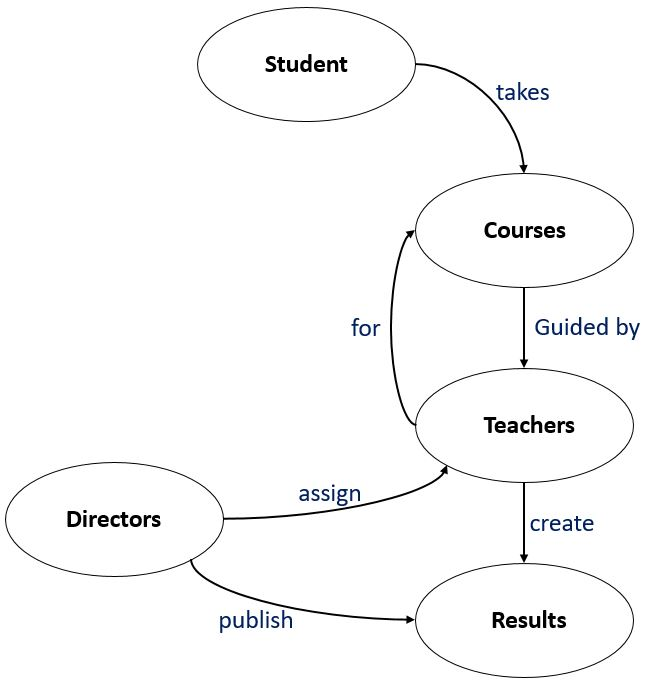
\includegraphics[width=10cm]{1.JPG}
    \caption{Entire work-flow}
    \label{fig:IICT WEBSITE}
\end{figure}
\newline
Figure 1.1 (Entire work-flow) is the overview of the project. Connection of all the entities are dependable to each others.  This gives the simple idea about the functional activities of the project. 
\newline
Student cycle, In the Figure 1.1 "Student" takes "Courses" ; "Courses" is guided by "Teachers"; "Teachers" creates "Results". 
\newline
Teacher cycle, In the Figure 1.1 "Director" assign "Teachers"; "Teachers" for particular "Courses"; "Director" publish "Results".
\newline
So, every entity is vary much interactive with each other.


\chapter{Projeto de Compiladores}

\section{Analise Léxica}
Antes de construirmos a gramática puramente dita, é necessário estabelecermos algumas considerações léxicas que são importantes para o funcionamento da linguagem DOGE\#. 
\par As palavras reservadas em DOGE\# são \textbf{if, while, print, return, int, char e void}. Essas palavras são terminais e são sempre representadas em letras minúsculas. Importante salientar que qualquer letra maiúsculas não será aceita pela linguagem e retorná um erro léxico pelo compilador. Além disso, palavras reservadas devem ser separadas por espaços em branco. Exemplo: ifwhile é um \textit{Id}.               
\par Comentários são iniciados por \$ e terminam no final de uma linha. os comentários devem sempre ser declarados linha por linha. 

\par Um caractere é qualquer símbolo na tabela ASCII que esteja entre os valores decimais de 32 a 126. Para armazenar uma aspas dupla deve-se primeiro colocar uma barra invertida “$\backslash$””. O mesmo vale para barra invertida “$\backslash\backslash$”. O tab será denotado por “$\backslash$t” e a quebra de linha por “$\backslash$n”. O caractere será delimitado sempre por aspas dupla (""). 
\par Números em DOGE\# são de 32 bit com sinal. Então, um número pode variar de -2147483648 até 2147483647. Um número muito grande será entendido como um número, porém dará erro somente na próxima análise.

\subsection{Gramática}
\par Nossa linguagem é construída sobre uma variação da Backus-Naur Form (BNF) denotada de Extended Backus-Naur Form (EBNF). No entanto, realizamos algumas alterações na notação original da EBNF com o propósito de elucidar as regras de produção da  nossa gramática. Por isso, vamos adotar a seguinte convenção:
\begin{itemize}
\item 'x' $\rightarrow$ Aspas simples significa que x é um terminal. Nome de terminais são sempre em minúsculo;
  
\item \textit{x} $\rightarrow$ Itálico significa que \textit{x} é um não-terminal. Todos os nomes não terminais começam com maiúsculo;

\item $\langle$\textit{x}$\rangle$ $\rightarrow$ Significa zero ou uma ocorrência de \textit{x}, ou seja, \textit{x} é opcional.
  
\item \textit{x\textsuperscript{*}} $\rightarrow$ Significa zero ou mais ocorrências de \textit{x};
  
\item \textit{x\textsuperscript{+}} $\rightarrow$ Significa um ou mais ocorrências de \textit{x};
  
\item \textit{x\textsuperscript{+},} $\rightarrow$ Um lista separada por vírgula de um ou mais \textit{x's} (vírgulas aparecem apenas entre \textit{x's});
  
\item  | $\rightarrow$ Separa alternativas de produção.

\item $\varepsilon$ $\rightarrow$ Significa vazio.
  
\end{itemize}

\par Iniciaremos a definição das regras de produção da referida gramática através símbolo inicial da EBNF, que representar a estrutura de um programa escrito em DOGE\#. Primeiro será mostrado a regra de produção da EBNF e logo a baixo a explicação dela.

\begin{center}
\textit{Program }$::=$\textit{ Decl}\textsuperscript{*}
\end{center}

\par Esse não-terminal indica que um programa em DOGE\# sempre inicia com zero ou mais ocorrências de \textit{Decl}. Dessa forma, o nosso compilador, ao tentar compilar um arquivo vazio, irá aceitá-lo como um programa válido, como é o caso de grande parte dos compiladores.

\begin{center}
\textit{Decl }$::=$\textit{ VarDecl} | \textit {FunctionDecl}
\end{center}

\par O não-terminal \textit{Decl} é definido como \textit{VarDecl} ou um \textit{FunctionDecl}, que significa respectivamente, uma declaração de variável ou uma declaração de função. Dessa maneira, um programa pode começar direto por uma declaração de variável ou por uma declaração de função.

\begin{center}
\textit{VarDecl }$::=$ \textit{Var} ';'
\end{center}

\par Uma declaração de variável, representada pelo não-terminal \textit{VarDecl}, é semelhante à declaração de variável da linguagem C, porém não é possível declarar mais de uma por linha.

\begin{center}
\textit{FunctionDecl }$::=$ \textit{Type} \textit{Id } '('\textit{ Argument }')'\textit{ Block} \newline |  'void' \textit{Id } '('\textit{ Argument }')'\textit{ Block} 
\end{center}

\par A declaração de uma função inicia-se com o tipo de retorno do método, que pode ter um tipo definido pelo não-terminal \textit{Type} ou pode ser terminal 'void', seguido pelo nome da função, pelo parâmetro e por fim, o corpo da função. 

\begin{center}
\textit{Var }$::=$\textit{ Type Id}
\end{center}

\par A produção acima gera cadeias que começam com o tipo da variável a ser declarada que possui o seu tipo definido pelo não-terminal \textit{Type}, seguido de um identificador que é o nome da variável. Lembrando que a dimensão de uma variável é sempre 1, pois não é possível declarar vetor ou matriz. 

\begin{center}
\textit{Argument }$::=$\textit{ Var}\textsuperscript{+}, | $\varepsilon$
\end{center}

\par O não-terminal \textit{Argument} é definido por uma ou mais sequencia de declarações de variável que tem o tipo de parâmetro e o nome da variável associada a ele, separadas por vírgulas.

\begin{center}
\textit{Type }$::=$ 'int' | 'char'
\end{center}

\par A regra de produção que define o não-terminal \textit{Type} pode ser um terminal 'int' ou 'char'.

\begin{center}
\textit{Id }$::=$\textit{ Alpha AlphaNum}\textsuperscript{*} 
\end{center}

\par Um \textit{Id} refere-se ao nome da variável ou função a ser declarada. Obrigatoriamente, o nome deve começar com uma letra do alfabeto, seguido de zero ou mais caracteres alfanuméricos.

\begin{center}
\textit{Alpha }$::=$ 'a' | 'b' | ... | 'z' 
\end{center}

\par Um não-terminal \textit{Alpha} é definido pelos caracteres terminais do alfabeto que vão de a até z. 

\begin{center}
\textit{AlphaNum }$::=$\textit{ Alpha }| \textit{Digit}
\end{center}

\par Um não-terminal \textit{AlphaNum} pode ser tanto um não-terminal \textit{Alpha} ou um \textit{Digit}.

\begin{center}
\textit{Digit }$::=$ '0' | '1' | ... | '9' 
\end{center}

\par Um \textit{Digit} é definido pelos números terminais de 0 à 9. 

\begin{center}
\textit{Call }$::=$\textit{ Id} '(' \textit{Actuals} ')' ';'
\end{center}

\par Um \textit{Call} é chamado dentro do não-terminal \textit{Stmt}. Essa regra de produção é responsável pela operação que chama uma função na nossa linguagem. Ela é definida por um \textit{Id}, que deve ser o mesmo nome da função a ser referenciada, seguida de um parâmetro dado pelo não-terminal \textit{Actuals}.

\begin{center}
\textit{Actuals }$::=$\textit{ Expr}\textsuperscript{+}, | $\varepsilon$
\end{center}

\par Um \textit{Actuals} é definido por uma ou mais \textit{Expr}, ou então vazio, significando que, não é necessário passar nenhum valor para função. 

\begin{center}
\textit{Block }$::=$ '\{' \textit{ VarDecl}\textsuperscript{*} \textit{ Stmt}\textsuperscript{*} '\}'
\end{center}

\par Na nossa linguagem, um \textit{Block} refere-se bloco de código em que os comandos são inseridos. Dentro desse bloco de código é possível declarar zero ou mais variáveis, além de ser permitido declarar zero ou mais instruções. 

\begin{center}
\textit{Stmt }$::=$\textit{ Location AssingOp Exrp} ';' |\textit{ Call} | 'if' '(' \textit{Exrp} ')'\textit{ Block} |  'while' '(' \textit{Exrp} ')'\textit{ Block} |  'print' '(' \textit{ Expr}\textsuperscript{+}, ')' ';' | 'return' < Expr > ';'
\end{center}

\par A definição \textit{Stmt} é um comando composto que gera os vários tipos de cadeias, que correspondem aos comandos da nossa linguagem bem como as funcionalidades dela. Comandos de impressão, seleção, repetição, término de método ou retorno de valor entre outros são definidos nessa regra de produção. 

\begin{center}
\textit{Expr }$::=$\textit{ Literal} |\textit{ Expr BinOp Expr} | \textit{ -Expr} | '(' \textit{Expr} ')'  
\end{center}

\par O não-terminal \textit{Expr} também é uma regra de produção composta, que possui várias cadeias de variação que representam as expressões suportadas pela linguagem DOGE\#. 

\begin{center}
\textit{Location }$::=$\textit{ Id}
\end{center}

\par Dentre as regras de produção apresentadas, temos ainda a \textit{Location}, que é definida por um \textit{Id} que representa o nome da variável que receberá um valor dentro de \textit{Stmt}.

\begin{center}
\textit{AssingOp }$::=$ '='
\end{center}

\par O não-terminal \textit{AssingOp} é uma produção que define o operador de atribuição igual.

\begin{center}
\textit{Literal }$::=$\textit{ IntLiteral} | \textit{ CharLiteral}
\end{center}

\par Um \textit{Literal} é um não-terminal utilizado para representar um valor fixo. Este valor fixo pode ser um inteiro ou um caractere.

\begin{center}
\textit{IntLiteral }$::=$\textit{ DecimalLiteral}
\end{center}

\par Um \textit{IntLiteral} é uma definição de \textit{Literal} que representa números inteiros por meio de um \textit{DecimalLiteral}.

\begin{center}
\textit{DecimalLiteral }$::=$\textit{ Digit Digit\textsuperscript{*}}
\end{center}

\par Um \textit{DecimalLiteral} é definido obrigatoriamente por um \textit{Digit} seguido de zero ou mais \textit{Digits}.

\begin{center}
\textit{CharLiteral }$::=$ '"' Char '"'
\end{center}

\par Este não-terminal também faz parte de um \textit{Literal}, no entanto é definido por um 'char' que é um caractere da tabela ASCII definido nas considerações léxicas na seção anterior. 

\begin{center}
\textit{BinOp }$::=$\textit{ ArithOp }|\textit{ RelOp }|\textit{ EqOp}
\end{center}

\par O não-terminal \textit{BinOp} é uma regra de produção composta, que pode ser definido por um \textit{ArithOp} ou \textit{RelOp} ou \textit{EqOp}.

\begin{center}
\textit{ArithOp }$::=$ '+'|'-'|'*'|'/'
\end{center}

\par O não-terminal \textit{ArithOp} é definido pelos operadores terminais de aritmética +,-,* e /. 

\begin{center}
\textit{RelOp }$::=$ '>'|'<'
\end{center}

\par O não-terminal \textit{RelOp} é definido pelos operadores terminais de relação > (maior) ou < (menor). 

\begin{center}
\textit{EqOp }$::=$ '=='|'!='
\end{center}

\par O não-terminal \textit{EqOp} é definido pelos operadores terminais de comparação == (igual) ou != (diferente). 

\subsection{Diagrama de Sintaxe}
Os diagramas de sintaxe representam a estrutura do programa em 
um formato que visa ser facilmente entendido, 
pois ao invés de ser escrito em texto, é apresentado de forma gráfica
facilitando assim a visualização do tipo de cadeias ou sentenças que 
cada nó não-terminal pode gerar. A representação por diagrama de sintaxe 
define para cada símbolo não-terminal um grafo direcionado com dois tipos de 
vértices: um vértice terminal e um vértice não-terminal. \par Esses grafos 
correspondem ao lado direito das produções da nossas gramatica na 
\textbf{BNF}, uma aresta de um nó \textit{A} para um nó \textit{B} indica que
que \textit{AB} é uma produção. Assim podemos dizer que a aresta indica a 
concatenação de duas cadeias. Todo grafo possui apenas um nó inicial, que 
não recebe nenhuma aresta e um único final de onde nenhuma aresta parte. Os símbolos não terminais são representados por retângulos.\par A representação por diagrama de sintaxe
para \textbf{DOGE\#} é a seguinte:
\begin{itemize}
\begin{center}
\item[$-$] \textit{Program}
	\begin{figure}[h]
	    \centering
		\begin{tikzpicture}
			\node[block]     (field) at (1,-1) {\textit{Decl}} ;
			
			\draw[thick,rounded corners=8pt,->]   (-2, 0)  -- (4, 0);
            \draw[thick,rounded corners=8pt,->]   (-1,0) -- (-1,-1) -- (field);
            \draw[thick,rounded corners=8pt,->]   (field) -- (3,-1) -- (3,0);
		\end{tikzpicture}
	\end{figure}
	
	\item[$-$] \textit{Decl}
	\begin{figure}[h]
	\centering
		\begin{tikzpicture}
			\node[block]     (varDecl)      at (-0.7,0) {\textit{VarDecl}} ;
			\node[block]     (functionDecl) at (2.6,-1) {\textit{FunctionDecl}} ;
			
			\draw[thick,rounded corners=8pt,->] (-2,0) -- (varDecl);
			\draw[thick,rounded corners=8pt,->] (varDecl) -- (6,0);
			\draw[thick,rounded corners=8pt,->] (0.6,0) -- (0.6,-1) -- (functionDecl);
			\draw[thick,rounded corners=8pt,->] (3.8,-1) -- (5,-1) -- (5,0);
		\end{tikzpicture}
	\end{figure}

    \item[$-$] \textit{VarDecl}
    \begin{figure}[h]
    \centering
		\begin{tikzpicture}
			\node[block] (var) at (1,-1) {\textit{Var}} ;
			
			\draw[thick,rounded corners=8pt,->] (-2, 0) -- (4, 0);
            \draw[thick,rounded corners=8pt,->] (-1,0) -- (-1,-1) -- (var);
            \draw[thick,rounded corners=8pt,->] (var) -- (3,-1) -- (3,0);
		\end{tikzpicture}
	\end{figure}
	
    \item[$-$] \textit{FunctionDecl}
    \begin{figure}[H]
    \centering
		\begin{tikzpicture}
			\node[block] (type)     at (-1,0)    {\textit{Type}};
            \node[sum]   (void)     at (-1,-1.5) {\textit{Void}};
            \node[block] (id)       at (1,0)     {\textit{Id}};
            \node[block] (bloco)    at (8,0)     {\textit{Block}};
            \node[sum]   (parEsq)   at (2.5,-1)  {(};
            \node[block] (Argum)    at (4.5,-1)  {\textit{Argument}};
            \node[sum]   (parDir)   at (6.5,-1)  {)};
            \node[block] (vazio)    at (4.5,-2)  {$\epsilon$};
			
			 \draw[thick,rounded corners=8pt,->] (-2,0)   -- (type);
             \draw[thick,rounded corners=8pt,->] (type)   -- (-2,-0.4) -- (-2,-1.5) -- (void); 
             \draw[thick,rounded corners=8pt,->] (void)   -- (0,-1.5)  -- (0,-0.4)  -- (type); 
             \draw[thick,rounded corners=8pt,->] (type)   -- (id);
             \draw[thick,rounded corners=8pt,->] (id)     -- (bloco);
             \draw[thick,rounded corners=8pt,->] (id)     -- (1.8,-0.05) -- (1.8,-1.2)  -- (parEsq);
             \draw[thick,rounded corners=8pt,->] (bloco)  -- (10,0);
             \draw[thick,rounded corners=8pt,->] (parEsq) -- (Argum);
             \draw[thick,rounded corners=8pt,->] (Argum)  -- (parDir);
             \draw[thick,rounded corners=8pt,->] (parDir) -- (7.1,-1.2) -- (7,-0.04) -- (bloco);
             \draw[thick,rounded corners=8pt,->] (Argum)  -- (3, -1.2) -- (3,-2) -- (vazio);
             \draw[thick,rounded corners=8pt,->] (vazio)  -- (6,-2) -- (6, -1.2) --  (Argum);
		\end{tikzpicture}
	\end{figure} 
	
	\item[$-$] \textit{Argument}
        \begin{figure}[H]
        \centering
            \begin{tikzpicture}
                \node[block] (var) at (1,-1) {\textit{Var}} ;
                \node[block] (vazio) at (1,-2) {\textit{Vazio}} ;
                
                \draw[thick,rounded corners=8pt,->] (-2, 0) -- (4, 0);
                \draw[thick,rounded corners=8pt,->] (-1,0)  -- (-1,-1) -- (var);
                \draw[thick,rounded corners=8pt,->] (var)   -- (3,-1) -- (3,0);
                \draw[thick,rounded corners=8pt,->] (var)   -- (-0.4, -1.4) -- (-0.4,-2) -- (vazio);
                \draw[thick,rounded corners=8pt,->] (vazio) -- (2,-2) -- (2, -1.2) --  (var);
            \end{tikzpicture}
        \end{figure} 
    
     \item[$-$] \textit{Var}
    \begin{figure}[h]
    \centering
		\begin{tikzpicture}
			\node[block] (var) at (-1,0) {\textit{Type}} ;
			\node[block] (id) at (1,-1) {\textit{Id}} ;
			
			\draw[thick,rounded corners=8pt,->] (-2, 0) -- (var);
            \draw[thick,rounded corners=8pt,->] (var) -- (4,0);
            \draw[thick,rounded corners=8pt,->] (-0.2, 0) -- (-0.2,-1) -- (id);
            \draw[thick,rounded corners=8pt,->] (id) -- (3,-1) -- (3,0);
		\end{tikzpicture}
	\end{figure}    

   \item[$-$] \textit{Type}
        \begin{figure}[H]
        \centering
            \begin{tikzpicture}
                \node[block] (var) at (1,-1) {\textit{Int}} ;
                \node[block] (vazio) at (1,-2) {\textit{char}} ;
                
                \draw[thick,rounded corners=8pt,->] (-2, 0) -- (4, 0);
                \draw[thick,rounded corners=8pt,->] (-1,0)  -- (-1,-1) -- (var);
                \draw[thick,rounded corners=8pt,->] (var)   -- (3,-1) -- (3,0);
                \draw[thick,rounded corners=8pt,->] (var)   -- (-0.4, -1.4) -- (-0.4,-2) -- (vazio);
                \draw[thick,rounded corners=8pt,->] (vazio) -- (2,-2) -- (2, -1.2) --  (var);
            \end{tikzpicture}
        \end{figure} 

    \item[$-$] \textit{Id}
    \begin{figure}[h]
    \centering
		\begin{tikzpicture}
			\node[block] (var) at (-1,0) {\textit{Alpha}} ;
			\node[block] (id) at (1,-1) {\textit{AlphaNum}} ;
			
			\draw[thick,rounded corners=8pt,->] (-2, 0) -- (var);
            \draw[thick,rounded corners=8pt,->] (var) -- (4,0);
            \draw[thick,rounded corners=8pt,->] (-0.2, 0) -- (-0.4,-1) -- (id);
            \draw[thick,rounded corners=8pt,->] (id) -- (3,-1) -- (3,0);
		\end{tikzpicture}
	\end{figure}    
	
	\item[$-$] \textit{Call}
    \begin{figure}[H]
    \centering
		\begin{tikzpicture}
			\node[block] (var) at (-1,0) {\textit{Id}} ;
			\node[sum] (a) at (0.5,-1) {(} ;
			\node[block] (b) at (2,-1) {\textit{Actuals}} ;
			\node[sum] (c) at (3.5,-1) {)} ;
			
			\draw[thick,rounded corners=8pt,->] (-2, 0) -- (var);
            \draw[thick,rounded corners=8pt,->] (var) -- (5,0);
            \draw[thick,rounded corners=8pt,->] (-0.2, 0) -- (-0.4,-1) -- (a);
            \draw[thick,rounded corners=8pt,->] (a) -- (b);
            \draw[thick,rounded corners=8pt,->] (b) -- (c);
            \draw[thick,rounded corners=8pt,->] (c) -- (4.5,-1) -- (4,0);
		\end{tikzpicture}
	\end{figure}
	
	\item[$-$] \textit{Actuals}
        \begin{figure}[H]
        \centering
            \begin{tikzpicture}
                \node[block] (var) at (1,-1) {\textit{Expr}} ;
                \node[block] (vazio) at (1,-2) {\textit{$\epsilon$}} ;
                
                \draw[thick,rounded corners=8pt,->] (-2, 0) -- (4, 0);
                \draw[thick,rounded corners=8pt,->] (-1,0)  -- (-1,-1) -- (var);
                \draw[thick,rounded corners=8pt,->] (var)   -- (3,-1) -- (3,0);
                \draw[thick,rounded corners=8pt,->] (-1,0)  -- (-1,-2) -- (vazio);
                \draw[thick,rounded corners=8pt,->] (vazio) -- (3,-2) -- (3,0);
            \end{tikzpicture}
        \end{figure} 
        
    \item[$-$] \textit{Stmt}
    \begin{figure}[H]
    \centering
		\begin{tikzpicture}
			\node[block]   (a)   at (-1,0)    {\textit{Location}};
            \node[block]   (b)   at (-2.5,0) {\textit{AssignOp}};
            \node[block]   (c)   at (4,0)     {\textit{Expr}};
            \node[block]   (d)   at (8,0)     {\textit{call}};
            \node[block]   (e)   at (2.5,-1)  {if};
            \node[block]   (f)   at (4.5,-1)  {\textit{while}};
            \node[block]   (g)   at (6.5,-1)  {print};
            \node[sum]     (h)   at (4.5,-2)  {return};
			
			 \draw[thick,rounded corners=8pt,->] (-2,0)   -- (type);
             \draw[thick,rounded corners=8pt,->] (type)   -- (-2,-0.4) -- (-2,-1.5) -- (void); 
             \draw[thick,rounded corners=8pt,->] (void)   -- (0,-1.5)  -- (0,-0.4)  -- (type); 
             \draw[thick,rounded corners=8pt,->] (type)   -- (id);
             \draw[thick,rounded corners=8pt,->] (id)     -- (bloco);
             \draw[thick,rounded corners=8pt,->] (id)     -- (1.8,-0.05) -- (1.8,-1.2)  -- (parEsq);
             \draw[thick,rounded corners=8pt,->] (bloco)  -- (10,0);
             \draw[thick,rounded corners=8pt,->] (parEsq) -- (Argum);
             \draw[thick,rounded corners=8pt,->] (Argum)  -- (parDir);
             \draw[thick,rounded corners=8pt,->] (parDir) -- (7.1,-1.2) -- (7,-0.04) -- (bloco);
             \draw[thick,rounded corners=8pt,->] (Argum)  -- (3, -1.2) -- (3,-2) -- (vazio);
             \draw[thick,rounded corners=8pt,->] (vazio)  -- (6,-2) -- (6, -1.2) --  (Argum);
		\end{tikzpicture}
	\end{figure} 
		
\end{center}
\end{itemize}

\subsection{Product Perspective}
"IICT WEBSITE" is the replacement of the manual hard copy result process. The data have been stored in the hard file or papers, this website will store all of those in the website. Main goal of this project is to minimize the work and maximize the result of this result processing system.

\section{User Classes and Characteristics}
"IICT WEBSITE" has basically 4 types of users. 
\begin{itemize}
  \item Teachers
    \begin{itemize}
        \item Director
        \item Course Teacher
    \end{itemize}
  \item Students
  \item Official Staff
\end{itemize}
Teacher has 2 types - Director defines the course teachers who will take the courses. Student fulfill all the requirements like- fees, informations can take advantages of the website. 
\begin{figure}
    \centering
    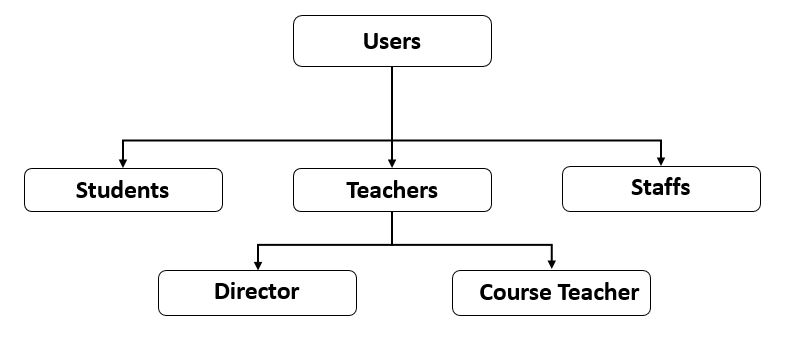
\includegraphics[width=10cm]{2.JPG}
    \caption{type of users}
    \label{fig:type of users}
\end{figure}

\section{Descrição de Comandos}
"IICT WEBSITE" store all the results of the students of program PGD, MIT. Also others programs can be included if necessary.
\begin{figure}[h!]
    \centering
    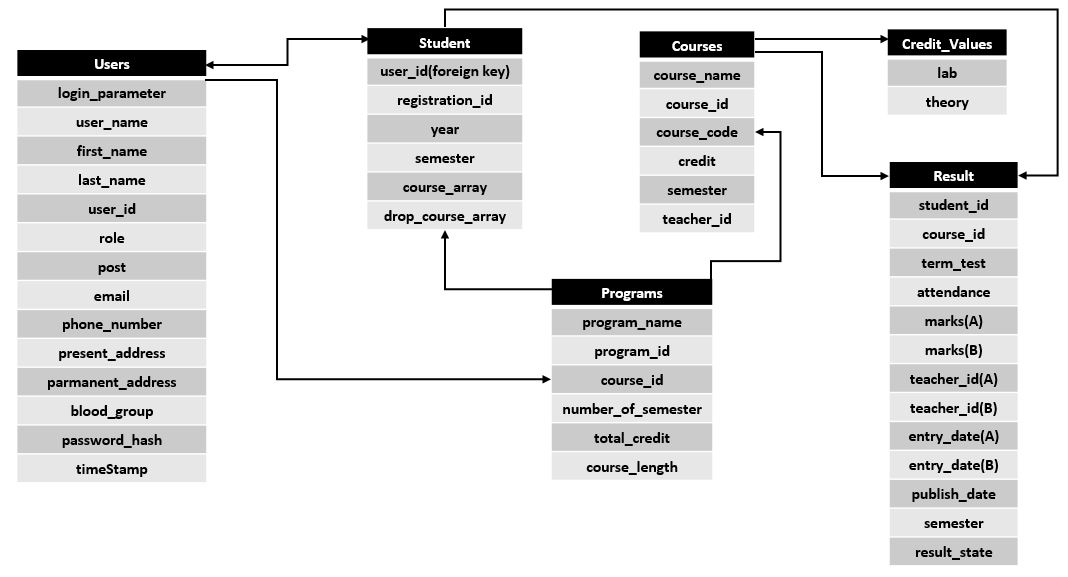
\includegraphics[width=15cm]{3.JPG}
    \caption{Data Flow Diagram}
    \label{fig:Data Flow Diagram}
\end{figure}
Before using the main function of the software result process, users have to be registered. 
\newline
All users have - login\_parameter, user\_name, first\_name, last\_name, user\_id, role, post, email, phone\_number, present\_address, parmanent\_address, blood\_group, password\_hash and timeStamp.
\newline
Students have some extra informations after complete his/her registration , such as - user\_id(foreign key), registration\_id, year, semester, course\_array and drop\_course\_array. These are the information that contains his/her result of his taken courses and program.
\newline
Each programs has some data - program\_name, program\_id, course\_id, nunmber\_of\_semester, total\_credit and course\_length. There will be onew or many course\_id in each programs.
\newline
Courses table contains - course\_name, course\_id, course\_code, credit, semester and teacher\_id.
\newline
Every course has its own Credit Values. Those have been 2 types - lab, theory.
\newline
Result is the main feature of all. It contains the values of all the exams of a particular student. It has data field - student\_id, course\_id, term\_test, attendance, marks(A), marks(B), teacher\_id(A), teacher\_id(B), entry\_date(A), entry\_date(B), publish\_date, semester	and result\_state.

\section{Operating Environment}
The website will be operate in any Operating Environment - Mac, Windows, Linux etc. 

\section{Design}
Student activities have 3 steps -
\begin{itemize}
    \item From Fill Up Process
    \item Courses Payment
    \item Student Profile
\end{itemize}
Top selected Student first fill his/her form, bank payment. After verification, student pays for their selected courses. Then he can enter his profile. 
\newline
Every student profile contains his/her personal information, results, taken courses, dropped courses and notice.
\newline
Notice will contain all the news of IICT.

\begin{figure}[h!]
    \centering
    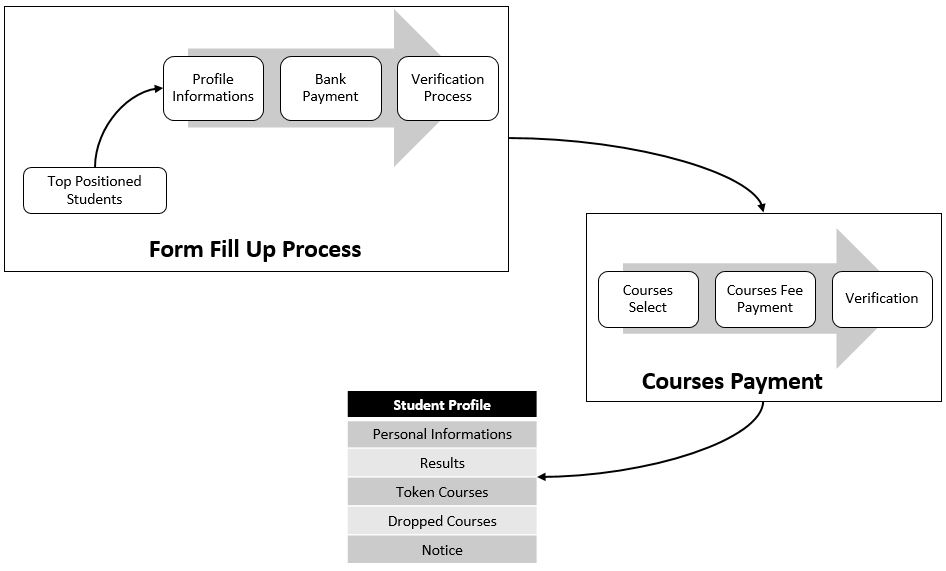
\includegraphics[width=15cm]{4.JPG}
    \caption{Student Activities}
    \label{fig:Students Activites}
\end{figure}
\newpage
Teacher activities have 2 steps - 
\begin{itemize}
    \item Director
    \item Course Teacher
\end{itemize}
Director can re-view the result, publish result, give notice and also create teacher. He can also perform course teacher activities.
\newline
Teacher creates results, view students and create notice.
\newline
\begin{figure}[h!]
    \centering
    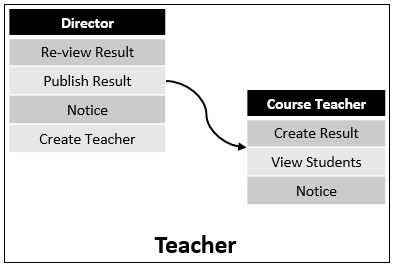
\includegraphics[width=10cm]{5.JPG}
    \caption{Teacher Activities}
    \label{fig:Teacher Activities}
\end{figure}
\newline
Staff has only one activity - 
\begin{itemize}
    \item Notice
\end{itemize} 
\begin{figure}[h!]
    \centering
    
\includegraphics[width=5cm]{6.JPG}
    \caption{Staff Activities}
    \label{fig:Staff Activities}
\end{figure}

\chapter{Analise Sintática}
"IICT WEBSITE" is a result processing web software. So the main art of this product is to enter data of results and publish. 

\section{Description and Priority}
"IICT WEBSITE" has features that are main and also some are sub. But all the feature is necessary for this software.
\newline
The features with priority up to down - 
\begin{enumerate}
    \item Result Creation : This is the goal feature of this software. It is been operated by teachers. They input the results of the students.
    \item Result Re-view : This is done by director.
    \item Result Publish : It is basically notice. This is mainly done by director or sometimes by staffs commanded by director.
    \item Teacher : Teacher takes the courses and create the results.
    \item Student : Student takes the courses of a program.
    \item Staff : Their only work is to post notice.
\end{enumerate}

\section{Functional Requirements}
The "IICT WEBSITE" website is being build on .NET framework, C\# language, React, React Redux, JavaScript and MongoDB.
\newline
Back-End - .NET framework, C\# language.
\newline
Font-End - React, React Redux, JavaScript.
\newline
Database -  MongoDB.


\chapter{Análise Semântica}

\section{Performance Requirements}
"IICT WEBSITE" will be used for result system of IICT programs, like - PGD, MIT. So for more interaction .NET, React and MongoDB is used. 

\section{Security Requirements}
No one without registered users can inter to the website. One particular user of a section only can perform his/her particular actions. 

\section{Software Quality Attributes}
In the development phase also testing and conferences of users is been continued. So that the quality of the software is been maintained and all the requirements are been fulfilled.
\newline
Database, logical and also UI test is required. 

\section{Business Rules}
"IICT WEBSITE" is for storing students results and publish those results of particular programs.
\newline
Basically save working time and pressure. 


\chapter{Other Requirements}
"IICT WEBSITE" needs maintenance as it is a long process software. It will need re-factoring and further the requirements can be changed as the field is changing frequently. 

\end{document}